% Inspired by Dan Spielman's template

\documentclass[10pt]{article}
\usepackage[T1]{fontenc}
\usepackage{amssymb}
\usepackage{amsmath}
\usepackage{graphicx}

\usepackage{tikz}
\usetikzlibrary{arrows,matrix}
\usepackage{subfigure}
\usepackage{stackrel}
\usepackage{blindtext}

\oddsidemargin=0.15in
\evensidemargin=0.15in
\topmargin=-.5in
\textheight=9in
\textwidth=6.25in

\usepackage[colorlinks=true,breaklinks,pdfpagemode=none,linkcolor=blue, urlcolor = blue, citecolor=blue]{hyperref}
\usepackage{enumerate}

%\usepackage{enumitem}
%\setlist{itemsep=0mm}

%\usepackage[usenames,dvipsnames]{pstricks}
%\usepackage{epsfig}
\usepackage{amsmath,amsfonts,amssymb,bm}
%\usepackage{pst-grad} % For gradients
%\usepackage{pst-plot} % For axes

% Enviroment definitions (add your own here)

\newtheorem{theorem}{Theorem}
\newtheorem{corollary}[theorem]{Corollary}
\newtheorem{lemma}[theorem]{Lemma}
\newtheorem{observation}[theorem]{Observation}
\newtheorem{proposition}[theorem]{Proposition}
\newtheorem{definition}[theorem]{Definition}
\newtheorem{claim}[theorem]{Claim}
\newtheorem{fact}[theorem]{Fact}

\newenvironment{proof}{\noindent{\bf Proof}\hspace*{1em}}{\qed\bigskip}

% New commands (add your own here)

\newcommand{\eps}{\varepsilon}
\newcommand{\bbR}{\mathbb{R}}
\newcommand{\hv}{\hat{v}}
\newcommand{\hL}{\hat{L}}
\newcommand{\hlambda}{\hat{\lambda}}
\newcommand{\homega}{\hat{\omega}}
\newcommand{\hp}{\hat{p}}
\newcommand{\hW}{\hat{W}}
\newcommand{\cK}{\mathcal{K}}
\newcommand{\qed}{\rule{7pt}{7pt}}
\newcommand{\cF}{\mathcal{F}}

\begin{document}

    \noindent
    \begin{center}

        \hrulefill

        \vspace{5pt}

        \makebox[\textwidth]{ {\bf AB IdeaLab, Competitive Programming Team, Fall 18--Spring 19} \hfill  February 8, 2019}
        \vspace{0pt}

        {\Large \hfill  Lecture 2: Data Structures\hfill}
        \vspace{10pt}

        {\large \hfill  American Computer Science League, February Contest\hfill}
        \vspace{10pt}

        \makebox[\textwidth]{ {\it Lecturer: Sanjit Bhat \hfill Editor: Alexander Sun} } % primary editor is the 'lecturer'

        \vspace{-3pt}
        \hrulefill
    \end{center}

In the modern era where data is being produced at a rapidly increasing
pace\footnote{With the Internet of Things, everything from a lightbulb
to your car is generating data.}
and being used for ever-increasing
applications\footnote{With Machine Learning, data-driven services like Google Translate and
FaceID reach billions of users each day},
we need fast ways of storing data.
Ideally, we could develop one data structure to hold all types of data
and perform all operations in the quickest time possible, however,
such a structure is currently nonexistent.
Instead, computer scientists need to be able to determine what
data structures to use in their specific problem.

For the purposes of ACSL, we will be studying four data structures
in the following lecture: stacks, queues, binary search trees, and
heaps/priority queues.
We will go through what each of them are, how they operate,
operations you can do on them, and the runtime complexity for each operation.
Hopefully, you will find the complexity analysis to be an interesting intellectual endeavor.
If not, you will end up seeing this stuff a lot more in intermediate--advanced CS
classes in college and in job interviews, so it's a good idea to start now.

\paragraph{Basics on runtime.}
Sample stuff

\paragraph{Stacks.}
Sample stuff.

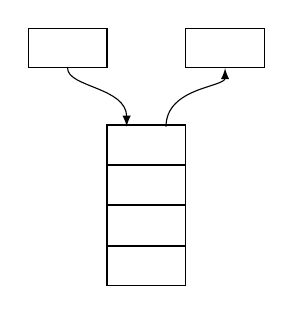
\begin{tikzpicture}[draw, minimum width=1cm, minimum height=0.5cm]
    \node[draw] (in) at (-1,2) {};
    \node[draw] (out) at (1,2) {};
    \matrix (queue)[matrix of nodes, nodes={draw, nodes={draw}}, nodes in empty cells]
    {
       \\ \\ \\ \\
    };

    \draw[-latex] (0.25,1) .. controls (0.25,1.5) and (1,1.5) .. (out.south);
    \draw[-latex] (in.south) .. controls (-1, 1.5) and (-0.25,1.5) .. (-0.25,1);
\end{tikzpicture}

\paragraph{Queues.}
Sample stuff.

\begin{tikzpicture}[draw, minimum width=1cm, minimum height=0.5cm]
    \node[draw] (in) at (-1,2) {};
    \node[draw] (out) at (1,-2) {};
    \matrix (queue)[matrix of nodes, nodes={draw, nodes={draw}}, nodes in empty cells]
    {
       \\ \\ \\ \\
    };

    \draw[-latex] (0.25,-1) .. controls (0.25,-1.25) and (1,-1.25) .. (out.north);
    \draw[-latex] (in.south) .. controls (-1, 1.5) and (-0.25,1.5) .. (-0.25,1);
\end{tikzpicture}

\paragraph{Binary search trees.}
Sample stuff.

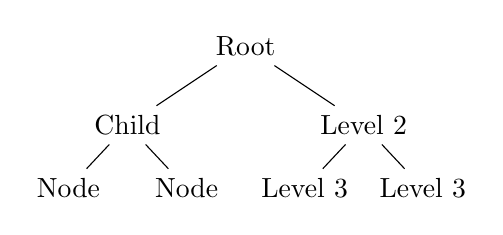
\begin{tikzpicture}[level distance=1.3cm,
   level 1/.style={sibling distance=3cm, level distance=1cm},
   level 2/.style={sibling distance=1.5cm, level distance=0.8cm}]
\node {Root}
   child {node {Child}
   child {node {Node}}
   child {node {Node}}
}
child {node {Level 2}
   child {node {Level 3}}
   child {node {Level 3}}
};
\end{tikzpicture}

\paragraph{Heaps/priority queues}
Sample stuff.

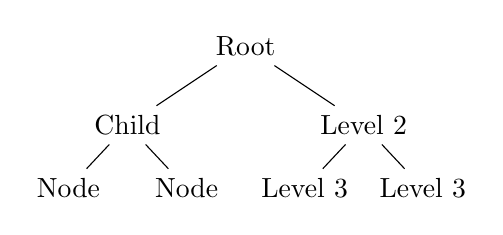
\begin{tikzpicture}[level distance=1.3cm,
   level 1/.style={sibling distance=3cm, level distance=1cm},
   level 2/.style={sibling distance=1.5cm, level distance=0.8cm}]
\node {Root}
   child {node {Child}
   child {node {Node}}
   child {node {Node}}
}
child {node {Level 2}
   child {node {Level 3}}
   child {node {Level 3}}
};
\end{tikzpicture}

\section{Exercises}
\begin{enumerate}
    \item
\end{enumerate}

\newpage
\section{Solutions}
\begin{enumerate}
    \item
\end{enumerate}

%\begin{thebibliography}{9}
%    \bibitem{deep_learning}
%    Lecun, Y., Bengio, Y., and Hinton, G. (2015).
%    Deep learning.
%    Nature, 521(7553), 436-444.
%\end{thebibliography}
\end{document}